\chapter{ESG swaps}


\section{ESG}
ESG \nomenclature{ESG}{Environmental, Social, and Governance} stands for Environmental, Social, and Governance. ESG metrics are becoming more critical for the financial sector in the European Union. The European Union have established a new taxonomy \cite{EU:2021} for sustainable activities. 
\\~\\
This taxonomy is put in place so that the EU can be carbon neutral by 2050, the goal is to help investors and companies contribute to the Paris Climate agreement. It will enable companies and issuers to access financing consistent with these goals.
\\~\\ 
One such contribution could be to access cheaper swap prices by meeting certain ESG criteria. Which in our case will be a particular ESG score. Let us take a look at what the different letters could represent:
\begin{itemize}
    \item Environmental: typically Climate risks, one metric could be $CO_{2}$-emissions. 
    \item Social: metrics could be: workforce rights, consumer protests etc. 
    \item Governance: management structure, diversity, crisis management, codes of conduct etc. 
\end{itemize}

We will not go into detail when it comes to the ESG risk score, as this would be a thesis in itself. However, we propose a model and show some implications. 

\newpage 

\section{Case study}
Our modelling approach will be based on the ISDA document \cite{ISDA:2021}, and in particular, the interest rate swap between SBM Offshore and ING, where the ESG score is set by Sustainalytics. The deal has the following specifications:
\begin{itemize}
    \item It gets added a positive or negative spread to the fixed rate set at the inception of the swap, based upon SBM's ESG score set by Sustainalytics. 
    \item At the beginning of every year during the life of the swap, ING set's a target ESG score.
    \item If the score has been met, then a discount of 5-10 basis points is applied to the fixed rate.
    \item If the score has not been met, then a penalty of 5-10 basis points is applied to the fixed rate. 
\end{itemize} 

In our simulation we will consider the ESG criteria to be $\F_{0}$-measurable, we will also take a constant discount $d$. To exemplify this deal pretend that the original fixed rate was set at $\kappa = 0.07$, with a discount/penalty $d = 0.005$ and the contract length is $n=4$ years. 
\\~\\
Assume that SBM Offshore met the criteria the first three times but did not meet the criteria the last time, that would given arise to the following ESG fixed rate sequence: 
\begin{align*}
K_{1}^{ESG} &=  0.065, \;\; 
K_{2}^{ESG} =   0.060, \;\;
K_{3}^{ESG} =   0.055, \;\; 
K_{4}^{ESG} =   0.060
\end{align*}


\begin{figure}[htp]
    \centering
    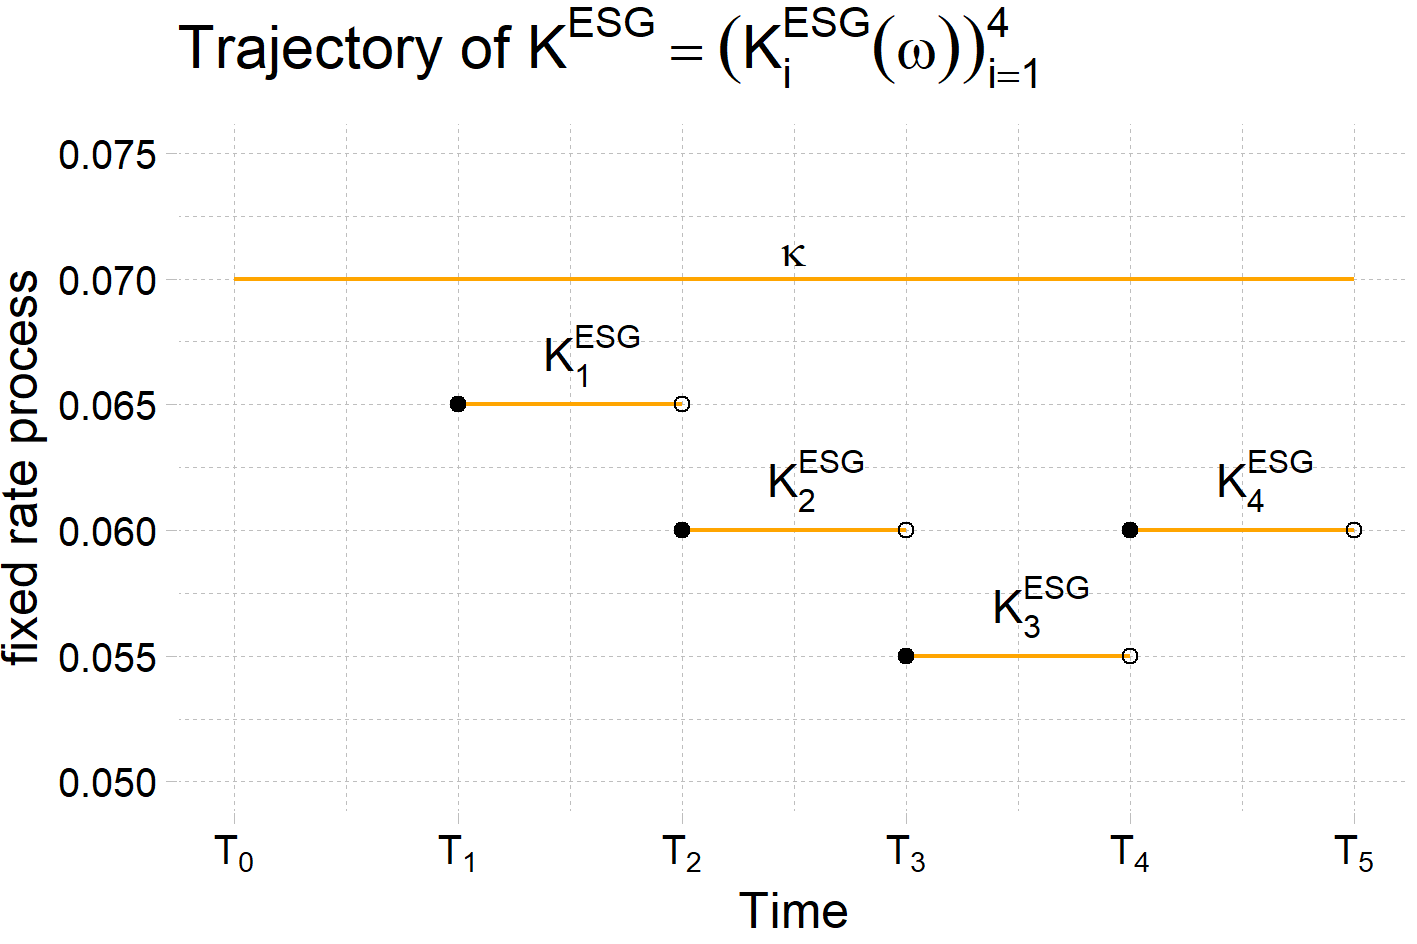
\includegraphics[width=12cm]{figures/ESG/SBM_ESG_path.png}
    \caption{ESG-fixed rate trajectory}
    \label{fig: SBM_ESG_path}
\end{figure}














\newpage 


\section{General setup}
We will take this deal as motivation, but generalize a bit further:
\begin{assumption}
We assume the following: 
\begin{itemize}[leftmargin=*]
    \item $N$ represents the nominal value, think of it as the amount you loan/lend.
    \item $0 < T_{0} < T_{1} < \dots < T_{n}$ a sequence of future dates. 
    \item $\delta = T_{i} - T_{i-1}$ a fixed leg between payments 
    \item $\kappa$ the fixed rate from the original swap, i.e without ESG-link. 
    \item $d$ basis points added or subtracted to the fixed rate $\kappa$
    \item $\{A_{i}\}_{i=1}^{n}$ sequence of events, where: 
    $A_{i} = \{X_{T_{i}} \leq C_{T_{i}}^{ESG}\}$ i.e the sequence of events measuring whether or not the ESG-criteria $C_{T_{i}}^{ESG}$ is met at time $T_{i}$ or not. 
\end{itemize}
\end{assumption} 


\begin{definition}[\textbf{ESG fixed rate process}]
Let $K^{ESG} = (K_{i}^{ESG})_{i=1}^{n}$ \nomenclature{$K^{ESG}$}{ESG fixed rate process}
denote the ESG fixed rate process, we define it recursively as: 
\begin{align*}
K_{i}^{ESG}(\omega) &= (K_{i-1}^{ESG}(\omega)-d)\mathbbm{1}_{A_{i}}(\omega)
+ (K_{i-1}^{ESG}(\omega)+d)\mathbbm{1}_{A_{i}^{C}}(\omega), \;\; i\geq 2
\end{align*}

where:
\begin{align*}
K_{1}^{ESG}(\omega) &= (\kappa - d)\mathbbm{1}_{A_{1}}(\omega)
+ (\kappa + d)\mathbbm{1}_{A_{1}^{C}}(\omega)    
\end{align*}
\end{definition} 

\begin{notation}
Let $\mathcal{I} = \{k_{1}, \dots, k_{n}\}$ represent an index set. Furthermore, let\\ 
$k_{1}< \dots < k_{l} < \dots < k_{m}< \dots < k_{n}$ We then define:
\begin{align*}
\left(
\bigcap_{i\in \mathcal{I}}A_{i}
\right)^{
\{(k_{1}, k_{l}, k_{m})\}
}
&= 
A_{k_{1}}^{C}\cap A_{k_{2}} \cap \dots\cap A_{k_{l}}^{C}\cap
A_{k_{l+1}}\cap \dots \cap A_{k_{m}}^{C}\cap A_{k_{m+1}}\cap \dots \cap A_{k_{n}}
\end{align*}
\end{notation}

\begin{result}
\label{prop/result: K_ESG_n}
Let $n \in \N_{2}:= \{k: k\geq 2, k\in \N\}$, consider the above situation. Let $\mathcal{I}_{n} = \{1, \dots, n\}$ and $\mathcal{I}_{2n}^{Even} = \{2, \dots, 2n\}$,
$(A_{i})_{i\in \mathcal{I}}$ denotes the event that the ESG criteria are met.
Let $j_{1} < j_{2} < \dots < j_{|\mathcal{I}_{\alpha}^{Even}|} \in \N$
furthermore $|\mathcal{I}_{2n}^{Even}|$ and $|\mathcal{I}_{n}|$ denotes the cardinality of the respective sets. 
\\~\\ 
We can then express $K_{n}^{ESG}(\omega)$ as:
\begin{align*}
K_{n}^{ESG}(\omega) &= 
[\kappa -dn]\mathbbm{1}\left[
\bigcap_{i\in \mathcal{I}_{n}}A_{i}
\right](\omega) \\ 
&+ 
\sum_{\alpha \in \mathcal{I}_{2n}^{Even}}
\left(
[\kappa -d(n-\alpha)]\mathbbm{1}\left[
\bigcup_{
j_{1}\neq \dots \neq j_{|\mathcal{I}_{\alpha}^{Even}|}
\in \mathcal{I}_{n}
}\left(
\bigcap_{i\in \mathcal{I}_{n}}A_{i}
\right)^{
\{
(j_{1}, \dots , j_{|\mathcal{I}_{\alpha}^{Even}|})
\}
}
\right]
\right)(\omega) 
\end{align*}
\end{result}  


\newpage 

To get a better grasp of Result \ref{prop/result: K_ESG_n}, we include the following graph: 
\begin{figure}[htp]
    \centering
    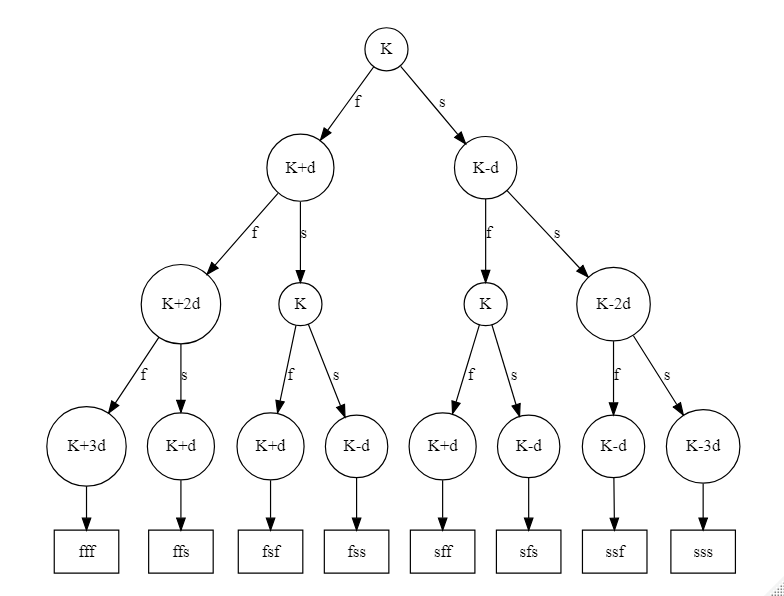
\includegraphics[width=13cm]{figures/ESG/tree_plt_ESG_seq.png}
    \caption{Possible outcomes of $K_{n}^{ESG}(\omega)$}
    \label{fig: Tree_plot_ESG_sequence}
\end{figure}

For a general $n$, we have $2^{n}$ possible paths, and the unique values will be
\begin{align*}
\kappa + id, i\in \{n-2k: k=0, \dots, n\}    
\end{align*}

We will have $|\{n-2k: k=0, \dots, n\}| = n + 1$ unique values. With ${n \choose |i|}$ number of possible paths leading to the value $\kappa + id$. 
\\~\\
Thus for $n = 3$, we have $2^{3} = 8$ possible paths, and $3+1 =4$ unique values: 
\begin{align*}
\kappa +3d, \; \kappa +d,\; \kappa -d\; \kappa - 3d    
\end{align*} 

We see that there are ${3 \choose 1} = 3$ different paths yielding a result of $\kappa +d$, which in this case are: $ffs, fsf$ and $sff$. 

\newpage 

\begin{align*}
K_{3}^{ESG}(\omega) &= 
[\kappa -3d]\mathbbm{1}\left[
\bigcap_{i\in \mathcal{I}_{3}}A_{i}
\right](\omega) \\ 
&+ 
\sum_{\alpha \in \{2,4,6\}}
\left(
[\kappa -d(3-\alpha)]\mathbbm{1}\left[
\bigcup_{\{
j_{1}\neq \dots \neq j_{|\mathcal{I}_{\alpha}^{Even}|}
\}
\in \{1,2,3\}
}\left(
\bigcap_{i =1}^{3}A_{i}
\right)^{
(j_{1}, \dots , j_{|\mathcal{I}_{\alpha}^{Even}|})
}
\right]
\right)(\omega) 
\end{align*}

The number of unique possible outcomes will be $|\{2,4,6\}| + 1 = 4$. If we fix $\alpha$, let's say, $\alpha = 4$, we get the value $\kappa +d$, and there are $3$ paths leading to this result. Now for $j_{1} < j_{2}$, we see that $j_{1} \neq j_{2} \in \{1,2,3\}$, leads to the following set-combinations: 
\begin{align*}
\{1,2\}, \; \{1,3\},\; \{2,3\}    
\end{align*}

Namely $3$ sets, where we got the index of where the criteria were not met. And this corresponds to the following expression: 

\begin{align*}
 &[\kappa - d(3-4)]\mathbbm{1}\left[
\bigcup_{j_{1}\neq j_{2}\in \{1,2,3\}}
\left[\bigcap_{i=1}^{3}A_{i}\right]^{\{(j_{1}, j_{2})\}}
\right](\omega) \\
= &[\kappa + d]\left[
\underbrace{
\mathbbm{1}(A_{1}^{C}\cap A_{2}^{C}\cap A_{3})(\omega)
}_{=ffs}
+ 
\underbrace{
\mathbbm{1}(A_{1}^{C}\cap A_{2}\cap A_{3}^{C})(\omega)
}_{=fsf} + 
\underbrace{
\mathbbm{1}(A_{1}\cap A_{2}^{C}\cap A_{3}^{C})(\omega)
}_{= sff}
\right]   
\end{align*}


\newpage 

\begin{proposition}
\label{prop: cond_expectation_ESG_sequence}
Let us denote $\kappa_{t}^{ESG}(i) := \E_{Q}[K_{i}^{ESG}(\omega)|\F_{t}]$. We then have\\ 
that for $t\leq T_{0}$ that: 
\begin{align*}
\kappa_{t}^{ESG}(i)
&= 
\kappa -d\cdot D(i)
\end{align*}

Where: 
\begin{align*}
 D(i) &= 
i\cdot \E_{Q}\left[
\prod_{l=1}^{i}\mathbbm{1}(A_{l})\bigg{|}\F_{t}
\right]
+ 
\sum_{\alpha \in \mathcal{I}_{2i}^{Even}}[i-\alpha]
\sum_{
j_{1}\neq \dots \neq j_{|\mathcal{I}_{\alpha}^{Even}|}
}
\E_{Q}\left[
\left(
\prod_{l=1}^{i}\mathbbm{1}(A_{l})
\right)^{
\{
(j_{1}, \dots , j_{|\mathcal{I}_{\alpha}^{Even}|})
\}
}
\bigg{|}\F_{t}
\right]   
\end{align*}
\end{proposition}

\begin{proof}

$K_{i}^{ESG}(\omega)$ is as described in Result \ref{prop/result: K_ESG_n}: 

\begin{align*}
\E_{Q}\left[K_{i}^{ESG}(\omega)
\bigg{|}\F_{t}\right]
&= 
[\kappa - d\cdot i]\E_{Q}\left[
\mathbbm{1}\left(
\bigcap_{l=1}^{i}A_{l}
\right)(\omega)\bigg{|}\F_{t}
\right] \\ 
&+
\sum_{\alpha \in \mathcal{I}_{2i}^{Even}}
\left(
[\kappa - d(i-\alpha)]
\E_{Q}\left[
\mathbbm{1}\left[
\bigcup_{\{
j_{1}\neq \dots \neq j_{|\mathcal{I}_{\alpha}^{Even}|}
\}
}
\left(
\bigcap_{l=1}^{i}
A_{l}
\right)
^{
\{
(j_{1}, \dots , j_{|\mathcal{I}_{\alpha}^{Even}|})
\}
}
\right](\omega)
\bigg{|}\F_{t}
\right]
\right)
\end{align*}

Now: 
\begin{align*}
&\E_{Q}\left[
\mathbbm{1}\left[
\bigcup_{\{
j_{1}\neq \dots \neq j_{|\mathcal{I}_{\alpha}^{Even}|}
\}
}
\left(
\bigcap_{l=1}^{i}
A_{l}
\right)^{
\{
(j_{1}, \dots , j_{|\mathcal{I}_{\alpha}^{Even}|})
\}
}
\right](\omega)
\bigg{|}\F_{t}
\right] \\
= 
\sum_{
j_{1}\neq \dots \neq j_{|\mathcal{I}_{\alpha}^{Even}|}
}
&\E_{Q}\left[
\mathbbm{1}\left(
\bigcap_{l=1}^{i}A_{l}
\right)^{
\{
(j_{1}, \dots, j_{|\mathcal{I}_{\alpha}^{Even}|})
\}
}
(\omega)
\bigg{|}\F_{t}
\right]
\end{align*}

Furthermore: 
\begin{align*}
\E_{Q}\left[
\mathbbm{1}\left(
\bigcap_{l=1}^{i}A_{l}
\right)(\omega)\bigg{|}\F_{t}
\right] 
&= \underbrace{
\E_{Q}\left[
\prod_{l=1}^{i}\mathbbm{1}(A_{l})\bigg{|}\F_{t}
\right]
}_{= s(l=1, i)}
\end{align*}

and:
\begin{align*}
\E_{Q}\left[
\mathbbm{1}\left(
\bigcap_{l=1}^{i}A_{l}
\right)^{
\{
(j_{1}, \dots, j_{|\mathcal{I}_{\alpha}^{Even}|})
\}
}(\omega)
\bigg{|}\F_{t}
\right] 
&= \underbrace{
\E_{Q}\left[
\left(
\prod_{l=1}^{i}\mathbbm{1}(A_{l})
\right)^{
\{
(j_{1}, \dots, j_{|\mathcal{I}_{\alpha}^{Even}|})
\}
}
(\omega)
\bigg{|}\F_{t}
\right]
}_{= f(l=1, i, j_{|\mathcal{I}_{\alpha}|})}
\end{align*}

\begin{align*}
\E_{Q}[K_{i}^{ESG}(\omega)|\F_{t}]
&= 
[\kappa -d\cdot i]s(l=1,i) \\
&+ 
\kappa \sum_{\alpha \in \mathcal{I}_{2i}^{Even}}
\sum_{
j_{1}\neq \dots \neq j_{|\mathcal{I}_{\alpha}^{Even}|}
}
f(l=1, i, j_{|\mathcal{I}_{\alpha}^{Even}|}) \\ 
&-
d\sum_{\alpha \in \mathcal{I}_{2i}^{Even}}
[i-\alpha]\sum_{
j_{1}\neq \dots \neq j_{|\mathcal{I}_{\alpha}^{Even}|}
}
f(l=1, i, j_{|\mathcal{I}_{\alpha}^{Even}|})
\end{align*}

\newpage 

We collect $\kappa$ and $d$-terms:
\begin{align*}
\E_{Q}[K_{i}^{ESG}(\omega)|\F_{t}]
&= 
\kappa
\underbrace{
\left[
s(l=1,i) + \sum_{\alpha \in \mathcal{I}_{2i}^{Even}}\sum_{
j_{1}\neq \dots \neq j_{|\mathcal{I}_{\alpha}^{Even}|}
}
f(l=1, i, j_{|\mathcal{I}_{\alpha}^{Even}|}) 
\right]
}_{=M(i)}
\\ 
&-d
\underbrace{
\left[
i\cdot s(l=1,i) + \sum_{\alpha \in \mathcal{I}_{2i}^{Even}}
\left(
[i-\alpha]\sum_{
j_{1}\neq \dots \neq j_{|\mathcal{I}_{\alpha}^{Even}|}
}
f(l=1, i, j_{|\mathcal{I}_{\alpha}^{Even}|})
\right)
\right]
}_{=D(i)} \\ 
&= 
\kappa M(i) -d\cdot D(i)
\end{align*}

Where: 
\begin{align*}
D(i) &= 
i\cdot \E_{Q}\left[
\prod_{l=1}^{i}\mathbbm{1}(A_{l})\bigg{|}\F_{t}
\right]
+ 
\sum_{\alpha \in \mathcal{I}_{2i}^{Even}}[i-\alpha]
\sum_{
j_{1}\neq \dots \neq j_{|\mathcal{I}_{\alpha}^{Even}|}
}
\E_{Q}\left[
\left(
\prod_{l=1}^{i}\mathbbm{1}(A_{l})
\right)^{
\{
(j_{1}, \dots , j_{|\mathcal{I}_{\alpha}^{Even}|})
\}
}
\bigg{|}\F_{t}
\right]
\end{align*}

and: 
\begin{align*}
M(i) &= 
\E_{Q}\left[
\prod_{l=1}^{i}\mathbbm{1}(A_{l})\bigg{|}\F_{t}
\right]  
+\sum_{\alpha \in \mathcal{I}_{2i}^{Even}}
\sum_{
j_{1}\neq \dots \neq j_{|\mathcal{I}_{\alpha}^{Even}|}
}
\E_{Q}\left[
\left(
\prod_{l=1}^{i}\mathbbm{1}(A_{l})
\right)^{
\{
(j_{1}, \dots , j_{|\mathcal{I}_{\alpha}^{Even}|})
\}
}
\bigg{|}\F_{t}
\right]
\end{align*}

Let's rewrite $M(i)$ on set notation again: 
\begin{align*}
M(i) &= 
\E_{Q}\left[
\mathbbm{1}\left(
\bigcap_{l \in \mathcal{I}_{i}}A_{l}
\right)
\bigg{|}\F_{t}
\right]
+\sum_{\alpha \in \mathcal{I}_{2i}^{Even}}
\E_{Q}\left[
\mathbbm{1}
\left[
\bigcup_{
j_{1} \neq \dots \neq j_{|\mathcal{I}_{\alpha}^{Even}|}
}
\left(
\bigcap_{l \in \mathcal{I}_{i}}A_{l}
\right)^{
\{
(j_{1}, \dots, j_{|\mathcal{I}_{\alpha}^{Even}|})
\}
}
\right]
\bigg{|}\F_{t}
\right]
\end{align*}

For $i = 1, \dots, n$, we have: 
\begin{align*}
\Omega_{i} 
&= 
\underbrace{
\left[
\sum_{\alpha \in \mathcal{I}_{2i}^{Even}}
\bigcup_{
j_{1} \neq \dots \neq j_{|\mathcal{I}_{\alpha}^{Even}|}
}
\left(
\bigcap_{l \in \mathcal{I}_{i}}A_{l}
\right)^{
\{
(j_{1}, \dots, j_{|\mathcal{I}_{\alpha}^{Even}|})
\}
}
\right]
}_{=\mathcal{H}_{i}}
\bigcup
\underbrace{
\left[
\bigcap_{l \in \mathcal{I}_{i}}A_{l}
\right]
}_{=\mathcal{L}_{i}}
\;\; 
\text{with}\;\; 
Q(\Omega_{i}) = 1
\end{align*} 

Now as $\mathcal{H}_{i}\cap \mathcal{L}_{i} = \emptyset$, 
and $\mathcal{H}_{i}\cup \mathcal{L}_{i} = \Omega_{i}$, in addition to exploiting the linearity of the expectation operator we get:

\begin{align*}
M(i) 
&= 
\E_{Q}\left[
\mathbbm{1}\left[
\left[
\sum_{\alpha \in \mathcal{I}_{2i}^{Even}}
\bigcup_{
j_{1} \neq \dots \neq j_{|\mathcal{I}_{\alpha}^{Even}|}
}
\left(
\bigcap_{l \in \mathcal{I}_{i}}A_{l}
\right)^{
\{
(j_{1}, \dots, j_{|\mathcal{I}_{\alpha}^{Even}|})
\}
}
\right]
\bigcup
\left[
\bigcap_{l \in \mathcal{I}_{i}}A_{l}
\right]
\right]
\bigg{|}\F_{t}
\right] \\ 
&= 
\E_{Q}\left[
\mathbbm{1}(\Omega_{i})|\F_{t}
\right] \\ 
&= 
1
\end{align*}

Leaving us with: 
\begin{align*}
\E_{Q}[K_{i}^{ESG}(\omega)|\F_{t}] &= 
\kappa - d\cdot D(i) := \kappa_{t}^{ESG}(i)
\end{align*}


\end{proof}


\section{Zero Coupon Bond ESG-swap}

\begin{proposition}
Consider a zero coupon bond swap, i.e where the situation is as described in Section \cref{sec: ZCB_swap}, we then get that the
\\ 
ESG-swap rate process $\kappa^{ESG}_{t} = (\kappa_{t}^{ESG}(i))_{i=1, \dots, n}$ is given by: 
\begin{align*}
\kappa_{t}^{ESG}(i) &= \kappa_{t}^{ZCB} -d\cdot D(i)    
\end{align*}
Where: 
\begin{align*}
\kappa_{t}^{ZCB} &=  
\frac{
P(t,T_{0}) - P(t,T_{n})
}{
\delta\sum_{i=1}^{n}P(t,T_{i})
}
\end{align*}
And $D(i)$ is as described in Proposition \ref{prop: cond_expectation_ESG_sequence}

\end{proposition}

\begin{proof}
Now from Section \cref{sec: ZCB_swap} we have that: 
\begin{align*}
\kappa_{t}^{ZCB} &=  
\frac{
P(t,T_{0}) - P(t,T_{n})
}{
\delta\sum_{i=1}^{n}P(t,T_{i})
}    
\end{align*}

Thus: 
\begin{align*}
\kappa_{t}^{ESG}(i) &= \kappa_{t}^{ZCB} -d\cdot D(i)    
\end{align*}
\end{proof}


